%include thesis.fmt

\hsdef{\begin{comment}
as,ds,f,ys,r,y,psi
supercompile,generalise,terminate
\end{comment}}
\begin{comment}
\begin{code}
import Prelude hiding (map,words,putStr,putChar)
import Data.List hiding (map,words)
import Data.Char
import GHC.Exts(build)

data Expr = EFun String [Expr]
          | EApp Expr [Expr]

freeVars :: Expr -> [String]
holes :: Expr -> [(Expr, Expr -> Expr)]
inline :: String -> Expr
terminate :: Expr -> Bool

data RealWorld = RealWorld
putStr :: String -> RealWorld -> (RealWorld, ())
putChar :: Char -> RealWorld -> (RealWorld, ())
\end{code}
\end{comment}


\chapter{Supercompilation}
\label{chp:supero}

This chapter deals with developing a \textit{supercompiler} for Haskell, which we have called Supero. We start with an introductory example in \S\ref{secS:intro_supero}, then describe our supercompilation method in \S\ref{secS:optimisation}. We then give a number of benchmarks, comparing both against C (compiled with GCC) in \S\ref{secS:c_results} and Haskell (compiled with GHC) in \S\ref{secS:haskell_results}. Finally, we review related work in \S\ref{secS:related}.

\section{Introductory Example}
\label{secS:intro_supero}

Haskell \cite{haskell} can be used in a highly declarative manner, to express specifications which are themselves executable. Take for example the task of counting the number of words in a file read from the standard input. In Haskell, one could write:

\begin{code}
main = print . length . words =<< getContents
\end{code}

From right to left, the |getContents| function reads the input as a list of characters, |words| splits this list into a list of words, |length| counts the number of words, and finally |print| writes the value to the screen.

An equivalent C program is given in Figure \ref{figS:c_words}. Compared to the C program, the Haskell version is more concise and more easily seen to be correct. Unfortunately, the Haskell program (compiled with GHC \cite{ghc}) is also three times slower than the C version (compiled with GCC). This slowdown is caused by several factors:

\begin{figure}
\begin{verbatim}
int main()
{
	int i = 0;
	int c, last_space = 1, this_space;
	while ((c = getchar()) != EOF) {
		this_space = isspace(c);
		if (last_space && !this_space)
			i++;
		last_space = this_space;
	}
	printf("%i\n", i);
	return 0;
}
\end{verbatim}
\caption{Word counting in C.}
\label{figS:c_words}
\end{figure}

\begin{description}
\item[Intermediate Lists] The Haskell program produces and consumes many intermediate lists as it computes the result. The |getContents| function produces a list of characters, |words| consumes this list and produces a list of lists of characters, |length| then consumes the outermost list. The C version uses no intermediate data structures.
\item[Functional Arguments] The |words| function is defined using the |dropWhile| function, which takes a predicate and discards elements from the input list until the predicate becomes true. The predicate is passed as an invariant function argument in all applications of |dropWhile|.
\item[Laziness and Thunks] The Haskell program proceeds in a lazy manner, first demanding one character from |getContents|, then processing it with each of the functions in the pipeline. At each stage, a lazy thunk for the remainder of each function is created.
\end{description}

Using Supero, we can eliminate all these overheads. We obtain a program that performs \textit{faster} than the C version. The optimiser is based around the techniques of supercompilation \cite{supercompilation}, where some of the program is evaluated at compile time, leaving an optimised residual program.

Our goal is an automatic optimisation that makes high-level Haskell programs run as fast as low-level equivalents, eliminating the current need for hand-tuning and low-level techniques to obtain competitive performance. We require no annotations on any part of the program, including the library functions.

\subsection{Contributions}

\begin{itemize}
\item To our knowledge, this is the first time supercompilation has been applied to Haskell.
\item We make careful study of the let expression, something absent from the Core language of many other papers on supercompilation.
\item We present an alternative generalisation step, based on a homeomorphic embedding \cite{leuschel:homeomorphic}.
\end{itemize}


\section{Supercompilation}
\label{secS:optimisation}

Our supercompiler takes a Core program as input, in the format described in \S\ref{secB:core}, and produces an equivalent Core program as output. To improve the program we do not make small local changes to the original, but instead \textit{evaluate it at compile time} so far as possible, leaving a \textit{residual program} to be run.

\begin{figure}
\ignore\begin{code}
supercompile()
    seen := {}
    bind := {}
    tie({}, main)

tie(rho, x)
    if x `notElem` seen then
        seen := seen `union` {x}
        bind := bind `union` {psi\!!(x) = \ freeVars\!!(x) -> drive\!!(rho,x)}
    {-" \textsf{\textbf{endif}} "-}
    {-" \textsf{\textbf{return }} "-} (psi\!!(x) freeVars\!!(x))

drive(rho, x)
    if terminate\!!(rho, x) then
        (cs,gen) = uniplate\!!(generalise\!!(x))
        {-" \textsf{\textbf{return }} "-} gen\!!(fmap (tie rho) cs)
    else
        {-" \textsf{\textbf{return }} "-} drive\!!(rho `union` {x}, unfold\!!(x))
\end{code}

Where |psi| is a mapping from expressions to function names, and \ignore|freeVars\!!(x)| returns the free variables in |x|. This code is parameterised by: |terminate| which decides whether to stop supercompilation of this expression; |generalise| which generalises an expression before residuation; |unfold| which chooses a function application and unfolds it.
\vspace{3mm}
\caption{The |supercompile| function.}
\label{figS:supercompile}
\end{figure}

The general method of supercompilation is shown in Figure \ref{figS:supercompile}. Each function in the output program is an optimised version of some associated expression in the input program. Supercompilation starts at the |main| function, and supercompiles the expression associated with |main|. Once the expression has been supercompiled, the outermost shell of the expression becomes part of the residual program -- making use of a Uniplate instance for our Core language (see Chapter \ref{chp:uniplate}). All the subexpressions are assigned names, and will be given definitions in the residual program. If any expression (up to $\alpha$-renaming) already has a name in the residual program, then the same name is used. Each of these named inner expressions is then supercompiled as before.

\begin{figure}
\ignore\begin{code}
case v of {... ; c vs_ -> x ; ...}
    => case v of {... ; c vs_ -> x[v/c vs_]; ...}

let v = x in y
    => y[v/x]
    where x {-" \hbox{ is a lambda or a variable } "-}

let v = c x_1 ... x_n in y
    =>  let v_1 = x_1 in
        ...
        let v_n = x_n in
        y[v/c x_1 ... x_n]
    where v_1 ... v_n {-" \hbox{ are fresh} "-}
\end{code}
\caption{Additional simplification rules.}
\label{figS:simplify}
\end{figure}

The supercompilation of an expression proceeds by repeatedly inlining a function application until some termination criterion is met. Once the termination criterion holds, the expression is generalised before the outer shell of the expression becomes part of the residual program and all subexpressions are assigned names. After each inlining step, the expression is simplified using the standard simplification rules from \S\ref{secB:core_simplify}, along with additional simplification rules from Figure \ref{figS:simplify}. The additional simplification rules all reduce the sharing in an expression, but by small constant amounts, and permit additional transformations. There are three key decisions in the supercompilation of an expression:

\begin{enumerate}
\item Which function to inline.
\item What termination criterion to use.
\item What generalisation to use.
\end{enumerate}

The original Supero work \cite{me:supero_ifl} inlined following evaluation order (with the exception of let expressions), used a bound on the size of the expression to ensure termination, and performed no generalisation. First we give examples of our supercompiler in use, then we return to examine each of the three choices we have made.

\subsection{Examples of Supercompilation}

\todo{Try and draw parallels between the Figure 4.2 and the example. Especially the unique-name stuff, but more too.}

\begin{examplename}{Supercompiling and Specialisation}

\begin{code}
main as = map (\b -> b + 1) as

map f cs = case  cs of
                 []    -> []
                 d:ds  -> f d : map f ds
\end{code}

There are two primary inefficiencies in this example: (1) the |map| function passes the |f| argument invariantly in every call; (2) the application of |f| is more expensive than if the function was known in advance.

The supercompilation proceeds by first assigning a new unique name (we choose |h_0|) to |map (\b -> b + 1) as|, providing parameters for each of the free variables in the expression, namely |as|. We then choose to expand |map|, and invoke the simplification rules:

\h{deflist}\begin{code}
h_0 as  = map (\b -> b + 1) as

        = case  as of
                []    -> []
                d:ds  -> d+1 : map (\b -> b + 1) ds
\end{code}

We now have a |case| with a variable as the scrutinee at the root of the expression, which cannot be reduced further, so we residuate the outer shell of the expression. When processing the expression |map (\b -> b + 1) ds| we spot this to be an $\alpha$-renaming of the body of an existing generated function, namely |h_0|, and use this function:

\begin{code}
h_0 as = case  as of
               []    -> []
               d:ds  -> d+1 : h_0 ds
\end{code}

We have now specialised the higher-order argument, passing less data at runtime.
\end{examplename}

\begin{examplename}{Supercompiling and Deforestation}

The deforestation transformation \cite{wadler:deforestation} removes intermediate lists from a traversal. A similar result is obtained by applying supercompilation, as shown here. Consider the operation of mapping |(*2)| over a list and then mapping |(+1)| over the result. The first |map| deconstructs one list, and constructs another. The second does the same.

\begin{code}
main as = map (\b -> b+1) (map (\c -> c*2) as)
\end{code}

We first assign a new name for the body of |main|, then choose to expand the outer call to |map|:

\begin{code}
h_0 as = case  map (\c -> c*2) as of
               []    -> []
               d:ds  -> d+1 : map (\b -> b+1) ds
\end{code}

Next we choose to inline the |map| scrutinised by the case, then perform the |case|/|case| simplification, and finally residuate:

\h{deflist}\begin{code}
h_0 as  = case  (case  as of
                       []    -> []
                       e:es  -> e*2 : map (\c -> c*2) es) of
                []    -> []
                d:ds  -> d+1 : map (\b -> b+1) ds

        = case  as of
                []    -> []
                d:ds  -> (d*2)+1 : map (\b -> b+1) (map (\c -> c*2) ds)

        = case  as of
                []    -> []
                d:ds  -> (d*2)+1 : h_0 ds
\end{code}

Both intermediate lists have been removed, and the functional arguments to |map| have both been specialised.
\end{examplename}

\subsection{Which function to inline}
\label{secS:which_inline}

During the supercompilation of an expression, at each step some function needs to be inlined. Which to choose? In most supercompilation work the choice is made following the runtime semantics of the program. But in a language with let expressions this may be inappropriate. If a function applied \textit{in a let binding} is inlined, its application when reduced may be simple enough to substitute in the let body. However, if a function applied \textit{in a let body} is inlined, the let body may now only refer to the let binding once, allowing the binding to be substituted. Let us take two expressions, based on intermediate steps obtained from real programs (word counting and prime number calculation respectively):

\begin{center}
\begin{tabular}{p{5cm}p{5cm}}
\h{expr}\begin{code}
let x = (==) $ 1
in x 1 : map x ys
\end{code}
&
\h{expr}\begin{code}
let x = repeat 1
in const 0 x : map f x
\end{code}
\end{tabular}
\end{center}

In the first example, inlining |($)| in the let binding gives |(\x -> 1 == x)|, which is now simple enough to substitute for |x|, resulting in |((1 == 1) : map (\x -> 1 == x) ys)| after simplification. Now |map| can be specialised appropriately. Alternatively, expanding the |map| repeatedly would keep increasing the size of expression until the termination criterion was met, aborting the supercompilation of this expression without achieving specialisation.

Taking the second example, |repeat| can be inlined indefinitely. However, by unfolding the |const| we produce |let x = repeat 1 in 0 : map f x|. Since |x| is only used once we substitute it to produce |(0 : map f (repeat 1))|, which can be deforested.

Unfortunately these two examples seem to suggest different strategies for unfolding -- unfold in the let binding or unfold in the let body. However, they do have a common theme -- unfold the function that cannot be unfolded infinitely often. Our strategy can be defined by the |unfold| function:

\begin{code}
unfold x = head (filter (not . terminate) xs ++ xs ++ [x])
    where xs = unfolds x

unfolds (EFun f xs_) = [ EApp (inline f) xs_ ]
unfolds x = [gen y | (c,gen) <- holes x, y <- unfolds c]
\end{code}

The |unfolds| function computes all possible one-step inlinings, using an in-order traversal of the abstract syntax tree, making use of the |holes| function defined by Uniplate in \S\ref{secU:holes_contexts}. The |unfold| function chooses the first unfolding which does not cause the supercompilation to terminate. If no such expression exists, the first unfolding is chosen.

\subsection{The Termination Criterion}

The original Supero program used a size bound on the expression to determine when to stop. The problem with a size bound is that different programs require different bounds to ensure both timely completion at compile-time and efficient residual programs. Indeed, within a single program, there may be different elements requiring different size bounds -- a problem exacerbated as the size and complexity of a program increases.

We use the homeomorphic embedding relation (described in \S\ref{secB:homeomorphic}). We terminate the supercompilation of an expression |y| if on the chain of reductions from |main| to |y| we have encountered an expression |x| such that $x \unlhd y$.

\todo{Define the additional termination criteria.}

In addition to using the homeomorphic embedding, we also terminate if further unfolding cannot yield any improvement to the root of the expression. For example, if the root of an expression is a constructor application, no further unfolding will change the root constructor. When terminating for this reason, we always residuate the outer shell of the expression, without applying any generalisation.

\subsection{Generalisation}

\todo{Separate into three different generalisation strategies. Give much better intuition.}

When the termination criterion has been met, it is necessary to discard information about the current expression, so that the supercompilation terminates. We always residuate the outer shell of the expression, but first we attempt to generalise the expression so that the information lost is minimal. The paper by \citet{sorensen:supercompilation} provides a method for generalisation, which works by taking the most specific generalisation of the current expression and an expression which is a homeomorphic embedding of it.

The most specific generalisation of two expressions $s$ and $t$, $\text{msg}(s,t)$, is produced by applying the following rewrite rule to the initial triple \linebreak $(x,\{x=s\},\{x=t\})$, resulting in a common expression and two sets of bindings.

\[
\left( \begin{array}{lcl}
	t_g \\
	\{x = \sigma(s_1,\ldots,s_n)\} & \cup & \theta_1 \\
	\{x = \sigma(t_1,\ldots,t_n)\} & \cup & \theta_2
	\end{array} \right)
\rightarrow
\left( \begin{array}{lcl}
	t_g[x / \sigma(y_1,\ldots,y_n)] \\
	\{y_1 = s_1,\ldots,y_n = s_n\} & \cup & \theta_1 \\
	\{y_1 = t_1,\ldots,y_n = t_n\} & \cup & \theta_2
	\end{array} \right)
\]

Our generalisation is characterised by $x \bowtie y$, which produces an expression equivalent to $y$, but similar in structure to $x$.

\ignore\begin{code}
{-" x \bowtie \sigma^*(y), \text{if dive}(x,\sigma^*(y)) \wedge \text{couple}(x,y) "-}
        let f = \vs_ -> x in {-" \sigma^* "-}(f vs_)
        {-" \text{where } "-}vs_{-" = \text{freeVars}(y) \backslash \text{freeVars}(\sigma^*(y)) "-}

{-" x \bowtie y, \text{if couple}(x,y) "-}
        let {-" \theta_2 "-} in {-" t_g "-}
        {-" \text{where }(t_g,\theta_1,\theta_2) = \text{msg}(x,y) "-}
\end{code}

The |freeVars| function in the first rule calculates the free variables of an expression, and $\sigma^*(y)$ denotes a subexpression $y$ within a containing context $\sigma^*$. The first rule applies if the homeomorphic embedding first applied the dive rule. The idea is to descend to the element which matched, and then promote this to the top-level using a lambda. The second rule applies the most specific generalisation operation if the coupling rule was applied first.

Some examples of our generalisation method, and the msg generalisation, are:

\begin{tabular}{@@{}r@@{ $\unlhd$ }l@@{\hspace{7mm}(}l@@{, }l@@{, }l@@{)\hspace{5.5mm} |let|\hspace{1mm}}l@@{\hspace{1mm}|in|\hspace{1mm}}l}
\multicolumn{2}{l}{\hspace{-2mm}Embedding} & \multicolumn{3}{l}{\hspace{-3mm}msg} & \multicolumn{2}{l}{\hspace{-7.5mm}$\bowtie$} \vspace{2mm} \\
$a$ & $b(a)$ & $x$ & $\{x = a\}$ & $\{x = b(a)\}$ & $f = b(a)$ & $f$ \\
$c(b)$ & $c(a(b))$ & $c(x)$ & $\{x = b\}$ & $\{x = a(b))\}$ & $x = a(b)$ & $c(x)$ \\
$b(a)$ & $c(b(a))$ & $x$ & $\{x = b(a)\}$ & $\{x = c(b(a))\}$ & $f = b(a)$ & $c(f)$
\end{tabular}

We now show an example where most specific generalisation fails to produce the ideal generalised version.

\begin{example}

\h{expr}\begin{code}
case  putStr (repeat '1') r of
      (r, _) -> (r, ())
\end{code}

This expression (which we name $x$) prints an infinite stream of 1's. The pairs and |r|'s correspond to the implementation of GHC's IO Monad \cite{spj:awkward_squad}. After several unrollings, we obtain the expression (named $x'$):

\h{expr}\begin{code}
case  putChar '1' r of
      (r, _) -> case  putStr (repeat '1') r of
                      (r, _) -> (r, ())
\end{code}

The homeomorphic embedding $x \unlhd x'$ matches, detecting an occurrence of the \ignore|case putStr \? ...| expression, and the supercompilation of $x'$ is stopped. The most specific generalisation rule is applied as $\text{msg}(x,x')$ and produces:

\h{expr}\begin{code}
let  a = putChar
     b = '1'
     c = \r -> case  putStr (repeat '1') r of
                     (r, _) -> (r, ())
in case  a b r of
         (r, _) -> c r
\end{code}

The problem is that msg works from the top, looking for a common root of both expression trees. However, if the first rule applied by $\unlhd$ was dive, the roots may be unrelated. Using our generalisation, $x \bowtie x'$:

\h{expr}\begin{code}
let x = \r -> case  putStr (repeat '1') r of
                    (r, _) -> (r, ())
in case  putChar '1' r of
         (r, _) -> x r
\end{code}

Our generalisation is superior because it has split out the |putStr| application \textit{without} lifting the |putChar| application or the constant |'1'|. The |putChar| application can now be supercompiled further in the context of the case expression.
\end{example}


\section{Performance Compared With C Programs}
\label{secS:c_results}

The benchmarks we have used as motivating examples are inspired by the Unix \texttt{wc} command -- namely character, word and line counting. We require the program to read from the standard input, and write out the number of elements in the file. To ensure that we test computation speed, not IO speed (which is usually determined by the buffering strategy, rather than optimisation) we demand that all input is read using the standard C \texttt{getchar} function only. Any buffering improvements, such as reading in blocks or memory mapping of files, could be performed equally in all compilers.

All the C versions are implemented following a similar pattern to Figure \ref{figS:c_words}. Characters are read in a loop, with an accumulator recording the current value. Depending on the program, the body of the loop decides when to increment the accumulator. The Haskell versions all follow the same pattern as in the Introduction, merely replacing |words| with |lines|, or removing the |words| function for character counting.

We performed all benchmarks on a machine running Windows XP, with a 3GHz processor and 1Gb RAM. All benchmarks were run over a 50Mb log file, repeated 10 times, and the lowest value was taken. The C versions used GCC\footnote{\url{http://gcc.gnu.org/}} version 3.4.2 with -O3. The Haskell version used GHC 6.8.1 with -O2. The Supero version was compiled using our optimiser, then written back as a Haskell file, and compiled once more with GHC 6.8.1 and -O2.

\begin{figure}
\bigskip
\begin{center}
% http://csdl.ics.hawaii.edu/FAQ/chart-ps.html
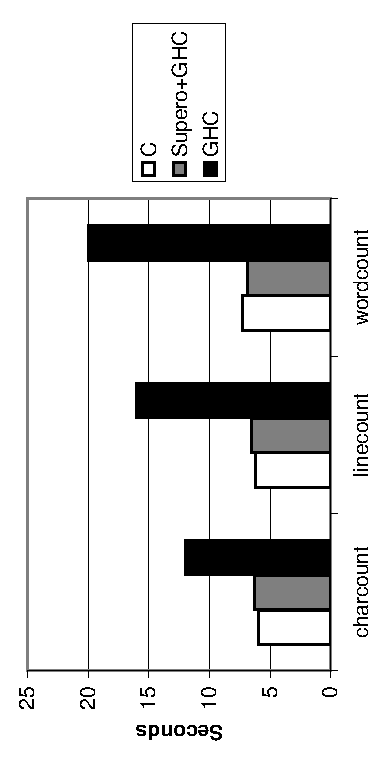
\includegraphics[scale=0.75,angle=270]{graphics/supero-wc.eps}
\end{center}
\bigskip
\caption{Benchmarks with C, Supero+GHC and GHC alone.}
\label{figS:c_results}
\end{figure}

The results are given in Figure \ref{figS:c_results}. In all the benchmarks C and Supero+GHC are within 10\% of each other, while GHC trails further behind.

\subsection{Identified Haskell Speedups}

During initial trials using these benchmarks, we identified two unnecessary bottlenecks in the Haskell version of word counting. Both were remedied before the presented results were obtained.

\paragraph{Slow \textsf{isSpace} function}

The first issue is that |isSpace| in Haskell is much more expensive than \texttt{isspace} in C. The simplest solution is to use a FFI (Foreign Function Interface) \cite{spj:awkward_squad} call to the C \texttt{isspace} function in all cases, removing this factor from the benchmark. A GHC bug (number 1473) has been filed about the slow performance of |isSpace|.

\begin{figure}
\begin{code}
words :: String -> [String]
words s = case  dropWhile isSpace s of
                []  ->  []
                x   ->  w : words y
                        where (w, y) = break isSpace x

words' s = case  dropWhile isSpace s of
                 []    ->  []
                 x:xs  ->  (x:w) : words' (drop1 z)
                           where (w, z) = break isSpace xs

drop1 []      = []
drop1 (x:xs)  = xs
\end{code}
\caption{The |words| function from the Haskell standard libraries, and an improved |words'|.}
\label{figS:words}
\end{figure}

\paragraph{Inefficient \textsf{words} function}

The second issue is that the standard definition of the |words| function (given in Figure \ref{figS:words}) performs two additional |isSpace| tests per word. By appealing to the definitions of |dropWhile| and |break| it is possible to show that in |words| the first character of |x| is not a space, and that if |y| is non-empty then the first character is a space. The revised |words'| function uses these facts to avoid the redundant |isSpace| tests.

\subsection{Potential GHC Speedups}

We have identified three factors limiting the performance of residual programs when compiled by GHC. These problems cannot be solved at the level of Core transformations. We suspect that by fixing these problems, the Supero execution time would improve by between 5\% and 15\%.

\paragraph{Strictness inference}

The GHC compiler is overly conservative when determining strictness for functions which use the FFI (GHC bug 1592). The \texttt{getchar} function is treated as though it may raise an exception, and terminate the program, so strict arguments are not determined to be strict. If GHC provided some way to mark an FFI function as not generating exceptions, this problem could be solved. The lack of strictness information means that in the line and word counting programs, every time the accumulator is incremented, the number is first unboxed and then reboxed \cite{spj:unboxing}.

\paragraph{Heap checks}

The GHC compiler follows the standard STG machine \cite{spj:stg} design, and inserts heap checks before allocating memory. The purpose of a heap check is to ensure that there is sufficient memory on the heap, so that allocation of memory is a cheap operation guaranteed to succeed. GHC also attempts to lift heap checks: if two branches of a case expression both have heap checks, they are replaced with one shared heap check before the case expression. Unfortunately, with lifted heap checks, a tail-recursive function that allocates memory only upon exit can have the heap test executed on every iteration (GHC bug 1498). This problem affects the character counting example, but if the strictness problems were solved, it would apply equally to all the benchmarks.

\paragraph{Stack checks}

The final source of extra computation relative to the C version are stack checks. Before using the stack to store arguments to a function call, a test is performed to check that there is sufficient space on the stack. Unlike the heap checks, it is necessary to analyse a large part of the flow of control to determine when these checks are unnecessary. It is not clear how to reduce stack checks in GHC.

\subsection{The Wordcount Benchmark}

The most curious result is that Supero outperforms C on wordcounting, by about 6\% -- even with the problems discussed! The C program presented in Figure \ref{figS:c_words} is not optimal. The variable \verb"last_space" is a boolean, indicating whether the previous character was a space, or not. Each time round the loop a test is performed on \verb"last_space", even though its value was determined and tested on the previous iteration. The way to optimise this code is to have two specialised variants of the loop, one for when \verb"last_space" is true, and one for when it is false. When the value of \verb"last_space" changes, the program would transition to the other loop. This pattern effectively encodes the boolean variable in the program counter, and is what the Haskell program has managed to generate from the high-level code.

However, in C it is quite challenging to capture the required control flow. The program needs two loops, where both loops can transition to the other. Using \texttt{goto} turns off many critical optimisations in the C compiler. Tail recursion is neither required by the C standard, nor supported by most compilers. The only way to express the necessary pattern is using nested while loops, but unlike newer imperative languages such as Java, C does not have named loops -- so the inner loop cannot break from the outer loop if it reaches the end of the file. The only solution is to place the nested while loops in a function, and use \texttt{return} to break from the inner loop. This solution would not scale to a three-valued control structure, and substantially increases the complexity of the code.

\section{Performance Compared With GHC Alone}
\label{secS:haskell_results}

The standard set of Haskell benchmarks is the nofib suite \cite{nofib}. It is divided into three categories of increasing size: imaginary, spectral and real. Even small Haskell programs increase in size substantially once libraries are included, so we have limited our attention to the benchmarks in the imaginary section. All benchmarks were run with parameters that require runtimes of between 3 and 5 seconds for GHC.

We exclude two benchmarks, paraffins and gen\_regexps. The paraffins benchmark makes substantial use of arrays, and we have not yet mapped the array primitives of Yhc onto those of GHC, which is necessary to run the transformed result. The gen\_regexps benchmark tests character processing: for some reason (as yet unknown) the supercompiled executable fails.

\begin{figure}
\bigskip
\begin{center}
% http://csdl.ics.hawaii.edu/FAQ/chart-ps.html
\includegraphics[scale=0.75,angle=270]{graphics/supero-nofib.eps}
\end{center}

\smallskip
\textbf{Supero} uses the $\bowtie$ generalisation method; \textbf{msg} uses the msg function for generalisation; \textbf{shell} applies no generalisation operation; \textbf{none} never performs any inlining. \\

\caption{Runtime, relative to GHC being 1.}
\label{figS:haskell_results}
\end{figure}

\begin{table}
\bigskip
\begin{tabular*}{\linewidth}{@@{\extracolsep{\fill}}lrrrrrr@@{\extracolsep{0cm}}}
\textbf{Program} & \textbf{Supero} & \textbf{msg} & \textbf{shell} & \textbf{none} & \textbf{Size} & \textbf{Memory} \\
bernouilli 		& 1.41 & 1.53 & 1.58 & 1.18 & 1.10 & 0.97 \\
digits-of-e1	& 1.03 & 1.16 & 1.03 & 1.06 & 1.01 & 1.11 \\
digits-of-e2	& 0.72 & 0.72 & 0.72 & 1.86 & 1.00 & 0.84 \\
exp3\_8			& 1.00 & 1.00 & 1.00 & 1.01 & 0.99 & 1.00 \\
integrate 		& 0.46 & 0.47 & 0.46 & 4.01 & 1.02 & 0.08 \\
primes 			& 0.57 & 0.57 & 0.88 & 0.96 & 1.00 & 0.98 \\
queens 			& 0.79 & 0.96 & 0.83 & 1.21 & 1.01 & 0.85 \\
rfib 			& 0.97 & 0.97 & 0.97 & 1.00 & 1.00 & 1.08 \\
tak 			& 0.72 & 1.39 & 1.39 & 1.39 & 1.00 & 1.00 \\
wheel-sieve1 	& 0.98 & 1.11 & 1.42 & 5.23 & 1.19 & 2.79 \\
wheel-sieve2 	& 0.87 & 0.63 & 0.89 & 0.63 & 1.49 & 2.30 \\
x2n1 			& 0.58 & 0.64 & 1.61 & 3.04 & 1.09 & 0.33 \\
\end{tabular*}
\bigskip

\textbf{Program} is the name of the program; \textbf{Supero} uses the $\bowtie$ generalisation method; \textbf{msg} uses the msg function for generalisation; \textbf{shell} applies no generalisation operation; \textbf{none} never performs any inlining; \textbf{Size} is the size of the Supero generated executable; \textbf{Memory} is the amount of memory allocated on the heap by the Supero executable. \\

\caption{Runtime, relative to GHC being 1.}
\label{tabS:haskell_results}
\end{table}

The results of these benchmarks are given in Figure \ref{figS:haskell_results}, along with detailed breakdowns in Table \ref{tabS:haskell_results}. All results are relative to the runtime of a program compiled with GHC -O2, lower numbers being better. The first three variants (Supero, msg, shell) all use homeomorphic embedding as the termination criterion, and $\bowtie$, msg or nothing respectively as the generalisation function. The final variant, none, uses a termination test that always causes a residuation. The `none' variant is useful as a control to determine which improvements are due to bringing all definitions into one module scope, and which are a result of supercompilation. Compilation times ranged from a few seconds to five minutes.

The Bernouilli benchmark is the only one where Supero is slower than GHC by more than 3\%. The reason for this anomaly is that a dictionary is referred to in an inner loop which is specialised away by GHC, but not by Supero.

With the exception of the wheel-sieve2 benchmark, our $\bowtie$ generalisation strategy performs as well as, or better than, the alternatives. While the msg generalisation performs better than the empty generalisation on average, the difference is not as dramatic.

\subsection{GHC's optimisations}

For these benchmarks it is important to clarify which optimisations are performed by GHC, and which are performed by Supero. The `none' results show that, on average, taking the Core output from Yhc and compiling with GHC does \textit{not} perform as well as the original program compiled using GHC. GHC has two special optimisations that work in a restricted number of cases, but which Supero-produced Core is unable to take advantage of.

\paragraph{Dictionary Removal} Functions which make use of type classes are given an additional dictionary argument. In practice, GHC specialises many such functions by creating code with a particular dictionary frozen in. This optimisation is specific to type classes -- a tuple of higher order functions is not similarly specialised. After compilation with Yhc, the type classes have already been converted to tuples, so Supero must be able to remove the dictionaries itself. One benchmark where dictionary removal is critical is digits-of-e2.

\paragraph{List Fusion} GHC relies on names of functions, particularly |foldr|/|build| \cite{spj:rules}, to apply special optimisation rules such as list fusion. Many of GHC's library functions, for example |iterate|, are defined in terms of |foldr| to take advantage of these special properties. After transformation with Yhc, these names are destroyed, so no rule based optimisation can be performed. One example where list fusion is critical is primes, although it occurs in most of the benchmarks to some extent.

\subsection{Compile Time}
\label{secS:compile_time}

The compile times for the benchmarks presented in Table \ref{tabS:haskell_results} vary between 1 minute and 12 minutes. These compile times are unsuitable for general development. Profiling shows that 25\% of the time is spent applying simplification rules, and 65\% is spent testing for a homeomorphic embedding. We suspect both these costs can be reduced, although we have not yet tried to do so.

\paragraph{Simplification Time} The rules from \S\ref{secB:core_simplify} are applied using the Uniplate library, in particular using the bottom-up rewrite strategy described in \S\ref{secU:rewrite_bottom}. After each function inlining, the rules are applied everywhere within the expression -- despite much of the expression remaining unchanged. By targeting the application of rules more precisely, compile times would decrease.

\paragraph{Homeomorphic Embedding} We use homeomorphic embedding to test a single element against a set of elements. The cost of homeomorphic embedding is related to the number of tests performed, and the size of the set at the time of each test. We perform many tests because of the unfolding strategy described in \S\ref{secS:which_inline}. The set is large because we maintain one set from the root function, including every inlining to the current point.

We have a solution -- split the homeomorphic embedding set in two. One set can be global and used for residuation, the other set can be local and used for inlining. Each expression is optimised within the context of a fresh local set, then for residuation the global set is used. The local set will be bounded by the number of inlinings since the last residuation, while the global set will be the number of residuations from the root function. These restrictions still ensure termination, and will decrease the size of the sets substantially. This scheme would permit more inlining steps to be performed, so would change the runtime performance, but we expect the effect to be positive.


\section{Related Work}
\label{secS:related}

\subsection{Supercompilation}

Supercompilation \cite{supercompilation,turchin:experiments} was introduced by Turchin for the Refal language \cite{refal}. Since this original work, there have been various suggestions of both termination strategies and generalisation strategies \cite{turchin:generalisation,sorensen:supercompilation,leuschel:homeomorphic}. The original supercompiler maintained both positive and negative knowledge, but our implementation is a simplified version maintaining only positive information \cite{secher:perfect_supercompilation}.

The issue of let expressions in supercompilation has not previously been a primary focus. If lets are mentioned, the usual strategy is to substitute all linear lets and residuate all others. Lets have been considered in a strict setting \cite{jonsson:supercompilation}, where they are used to preserve termination semantics, but in this work all strict lets are inlined without regard to loss of sharing. Movement of lets can have a dramatic impact on performance: carefully designed let-shifting transformations give an average speedup of 15\% in GHC \cite{spj:letfloating}, suggesting let expressions are critical to the performance of real programs.

\subsection{Partial evaluation}

\todo{Say what is the difference between supercompilation and partial evaluation}

There has been a lot of work on partial evaluation \cite{jones:partial_evaluation}, where a program is specialised with respect to some static data. The emphasis is on determining which variables can be entirely computed at compile time, and which must remain in the residual program. Partial evaluation is particularly appropriate for specialising an interpreter with an expression tree to generate a compiler automatically, often with an order of magnitude speedup, known as the First Futamura Projection \cite{futanama:projections}. Partial evaluation is not usually able to remove intermediate data structures. Our method is certainly less appropriate for specialising an interpreter, but in the absence of static data, is still able to show improvements.

% Partial evaluation has been applied to full-scale functional languages, such as Curry
% \cite{albert:partial_evaluation_curry}.

\subsection{Deforestation}

The deforestation technique \cite{wadler:deforestation} removes intermediate lists in computations. This technique has been extended in many ways to encompass higher order deforestation \cite{marlow:higher_order_deforestation} and work on other data types \cite{coutts:string_fusion}. Probably the most practically motivated work has come from those attempting to restrict deforestation, in particular shortcut deforestation \cite{gill:shortcut_deforestation}, and newer approaches such as stream fusion \cite{coutts:stream_fusion}. In this work certain named functions are automatically fused together. By rewriting library functions in terms of these special functions, fusion occurs.

\subsection{Whole Program Compilation}

The GRIN approach \cite{grin} uses whole program compilation for Haskell. It is currently being implemented in the jhc compiler \cite{jhc}, with promising initial results. GRIN works by first removing all functional values, turning them into case expressions, allowing subsequent optimisations. The intermediate language for jhc is at a much lower level than our Core language, so jhc is able to perform detailed optimisations that we are unable to express.

\subsection{Lower Level Optimisations}

Our optimisation works at the Core level, but even once efficient Core has been generated there is still some work before efficient machine code can be produced. Key optimisations include strictness analysis and unboxing \cite{spj:unboxing}. In GHC both of these optimisations are done at the Core level, using a Core language extended with unboxed types. After this lower level Core has been generated, it is then compiled to STG machine instructions \cite{spj:stg}, from which assembly code is generated. There is still work being done to modify the lowest levels to take advantage of the current generation of microprocessors \cite{marlow:pointer_tagging}. We rely on GHC to perform all these optimisations after Supero generates a residual program.

\subsection{Other Transformations}

One of the central operations within our optimisation is inlining, a technique that has been used extensively within GHC \cite{spj:inlining}. We generalise the constructor specialisation technique \cite{spj:specconstr}, by allowing specialisation on any arbitrary expression, including constructors.

One optimisation we do not currently support is the use of user provided transformation rules \cite{spj:rules}, which can be used to automatically replace certain expressions with others -- for example |sort . nub| removes duplicates then sorts a list, but can be done asymptotically faster in a single operation.

